%!TEX root = bare_conf.tex

\section{Setup} \label{sec:setup}
%TODO ros, caffe, gazebo, actions

Our system consist two major parts: the DQN and the simulation. Gazebo\footnote{\url{http://gazebosim.org}} is used as the simulation environment. And Caffe\cite{jia2014caffe} is selected as deep learning framework. Ros\footnote{\url{http://www.ros.org}} is chosen as a tool for the communication between DQN and Gazebo. We utilize a single normal camera as the unique sensor of the car. The system has five fixed actions, namely \textit{Left}, \textit{Half-left}, \textit{Straight}, \textit{Half-right} and \textit{Right}. The speed of all the five actions are same and will remain unchanged during the training. The DQN takes the images(in gray scale and resolution is $ 48 \times 27 $ pixels) from the camera as input and returns Q-values for all the five actions by a update rate of $ 200 Hz $. The action whose Q-value is largest will be selected as the one to be carried out by the car. The architecture is showed in Figure \ref{fig:archi}.

\begin{figure}[!t]
	\centering
	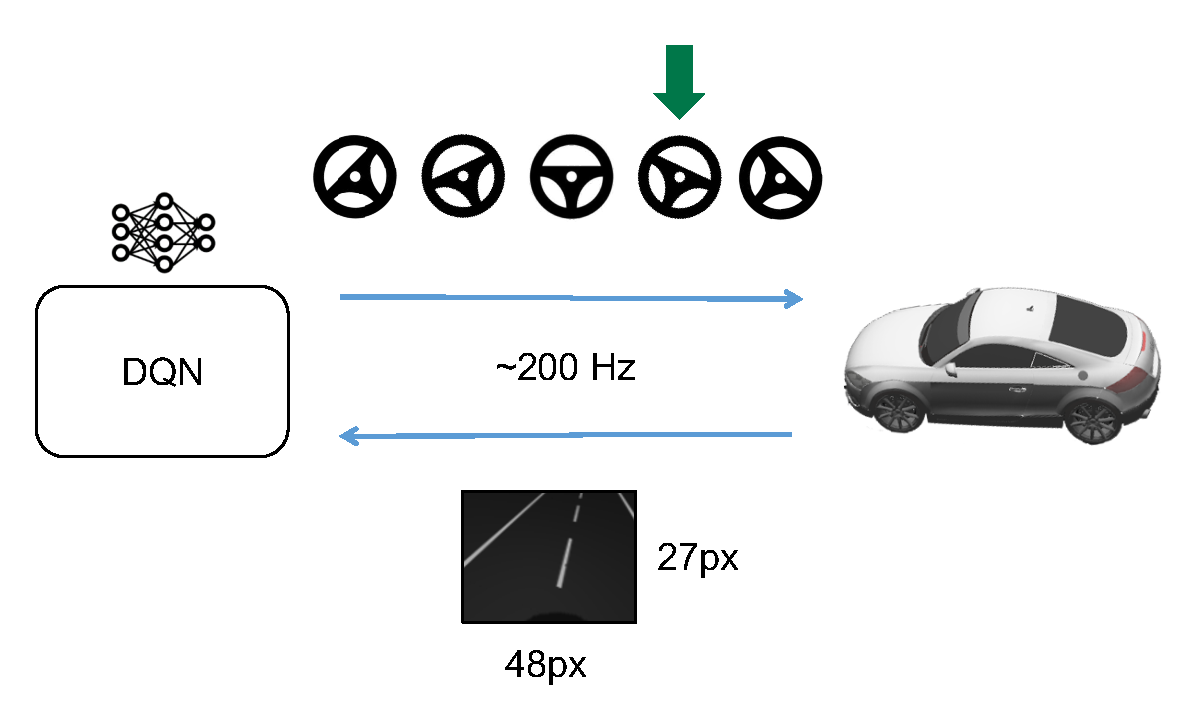
\includegraphics[width=3.5in]{../presentation/archi} 
	\caption{System architecture: Every time the Gazebo( showed as a car here) gives an image to DQN. DQN returns Q-values of the five actions according to the image it received. And the action with largest Q-value will be select as next action of the car. As an example here the action: \textit{Half-right} is selected.}
	\label{fig:archi}
\end{figure}